\documentclass[10pt,a4paper]{article}
\usepackage[utf8]{inputenc}
\usepackage[T1]{fontenc}
\usepackage{lmodern}
\usepackage[margin=1.4cm,top=1.45cm,bottom=1.45cm]{geometry}
\usepackage{amsmath,amssymb}
\usepackage{booktabs}
\usepackage{tabularx}
\usepackage{array}
\usepackage{enumitem}
\usepackage{float}
\usepackage[table]{xcolor}
\usepackage{colortbl}
\usepackage{tikz}
\usetikzlibrary{shapes.geometric,arrows.meta,positioning,fit,calc,backgrounds}
\usepackage{fancyhdr}
\usepackage{titlesec}
\usepackage{microtype}
\usepackage[colorlinks=true,linkcolor=blue!70!black,citecolor=blue!70!black,urlcolor=blue!70!black]{hyperref}

\newcolumntype{L}[1]{>{\raggedright\arraybackslash}p{#1}}
\newcolumntype{Y}{>{\raggedright\arraybackslash}X}
\newcommand{\sub}[1]{{\fontsize{5.5}{6}\selectfont\mdseries #1}}

% Header and Footer styling
\pagestyle{fancy}
\fancyhf{}
\fancyhead[L]{\small\textsf{\textbf{Part 1: The Twin} \textbar\ 3-Layer Urban IoT Monitoring Platform}}
\fancyhead[R]{\small\textsf{Page \thepage}}
\fancyfoot[L]{\small\textsf{Twin Layer Report \textbar\ Version 1.0}}
\fancyfoot[R]{\small\textsf{Signed telemetry \textbar\ Ground truth}}
\renewcommand{\headrulewidth}{0.5pt}
\renewcommand{\footrulewidth}{0.5pt}

% Section formatting
\titleformat{\section}
  {\normalfont\sffamily\Large\bfseries\color{blue!80!black}}
  {\thesection}{0.8em}{}
\titleformat{\subsection}
  {\normalfont\sffamily\large\bfseries\color{blue!70!black}}
  {\thesubsection}{0.6em}{}
\titleformat{\subsubsection}
  {\normalfont\sffamily\normalsize\bfseries\color{black}}
  {\thesubsubsection}{0.5em}{}

\titlespacing*{\section}{0pt}{4pt}{2pt}
\titlespacing*{\subsection}{0pt}{3pt}{1.5pt}
\titlespacing*{\subsubsection}{0pt}{2pt}{1pt}
\setlength{\parskip}{1pt}
\setlength{\parindent}{0pt}
\setlength{\intextsep}{4pt plus 1pt minus 1pt}
\setlength{\textfloatsep}{4pt plus 1pt minus 1pt}
\setlength{\abovecaptionskip}{2pt}
\setlength{\belowcaptionskip}{1.5pt}

\begin{document}

\setcounter{section}{0} % Starts section numbering at 1

\section{The Twin}

\subsection{Role and goals}
The Twin is the city. It simulates 42 field devices across six zones of Greater Tunis (Downtown Financial, Port \& Coastal Harbor in La Goulette, North Industrial Park, West Residential Hills, Central University \& Med, South Logistics Hub). Every zone has the same seven devices: two traffic cameras, two water-level floats, one power-load meter, one air-quality station and one emergency-call counter. Each device reports ten times per second, so the city streams about 420 signed readings per second whether or not anything is happening.

The Twin answers one question for its partners: \emph{what is happening in the city right now?} It has three jobs:
\begin{enumerate}[leftmargin=*,itemsep=0pt,topsep=1pt]
  \item \textbf{Stream telemetry.} Publish every reading to Kafka, signed with the device's own Ed25519 key, in a fixed and documented format of at most 300 bytes.
  \item \textbf{Accept commands.} Expose the city's actuators (dispatch units, traffic signal plans, drainage valves, grid switching) and its containment controls (isolate, quarantine, reinstate, release, roll back a reading) as 16 MCP tools. A command changes the simulated physics, so a good decision visibly helps the city and a bad one does not.
  \item \textbf{Be attackable, and keep the truth.} An adversary engine can spoof, replay, delay, corrupt or drop readings, plant a rogue device, steal a device key, freeze a sensor or make an actuator lie. The real physical state goes to a separate ground-truth ledger that no partner can read, so every scenario can be scored afterwards against what really happened.
\end{enumerate}
\textit{Goals we hold ourselves to:} a partner connects without reading our code (a one-page interface card, settings only, no hard-coded addresses); every scenario starts with one command and leaves a log; the same seed always gives the same physics; nothing a partner sends can crash the Twin or leak the ground truth.
\textit{Scope:} physics, incidents, attacks, signing, the Kafka stream, the MCP command surface, the ground-truth ledger, the operations console and the scenario runner. Out of scope: detecting incidents and choosing responses (Brain), judging whether data can be trusted (Guardian).

\subsection{Architecture}
Figure~\ref{fig:twin_arch} shows the Twin as it runs: one Python process with two network faces, Kafka going out and MCP coming in, plus a separate red-team port that partners never see.

\begin{figure}[H]
\centering
\resizebox{0.93\textwidth}{!}{%
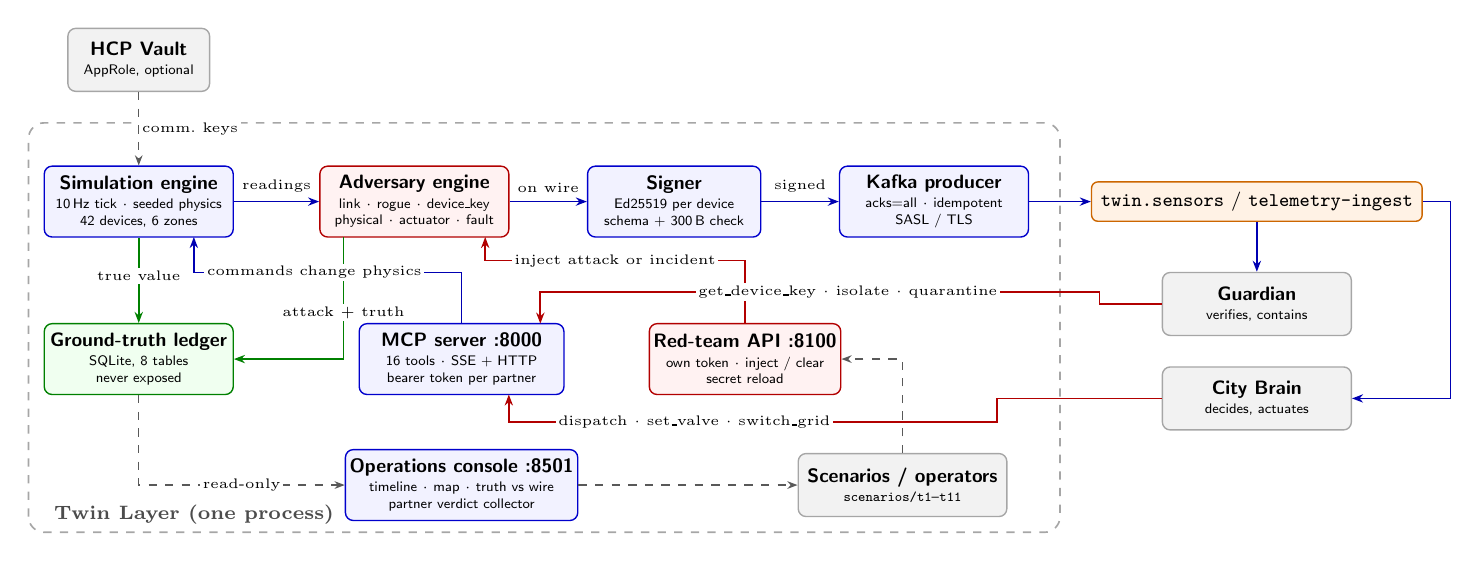
\begin{tikzpicture}[
    font=\sffamily\scriptsize,
    every node/.style={align=center},
    box/.style={rectangle, draw=blue!80!black, fill=blue!5!white, rounded corners=1mm, line width=0.5pt, inner sep=1.5pt, minimum height=0.9cm},
    adv/.style={rectangle, draw=red!70!black, fill=red!5!white, rounded corners=1mm, line width=0.5pt, inner sep=1.5pt, minimum height=0.9cm},
    store/.style={rectangle, draw=green!50!black, fill=green!6!white, rounded corners=1mm, line width=0.5pt, inner sep=1.5pt, minimum height=0.9cm},
    topic/.style={rectangle, draw=orange!80!black, fill=orange!10!white, rounded corners=0.8mm, minimum height=0.5cm, minimum width=3.4cm, line width=0.5pt},
    ext/.style={rectangle, draw=gray!70, fill=gray!10!white, rounded corners=1mm, line width=0.5pt, minimum height=0.8cm},
    lab/.style={font=\fontsize{5.5}{6}\selectfont, fill=white, inner sep=1pt},
    flow/.style={-{Stealth[scale=0.7]}, draw=blue!70!black, line width=0.6pt},
    rej/.style={-{Stealth[scale=0.7]}, draw=red!70!black, line width=0.6pt},
    aux/.style={-{Stealth[scale=0.7]}, draw=gray!70!black, dashed, line width=0.5pt}
]
% Twin boundary
\draw[dashed, rounded corners=2mm, gray!70, line width=0.6pt] (-0.5,-0.6) rectangle (12.6,4.6);
\node[anchor=west, font=\bfseries\scriptsize, text=gray!60!black] at (-0.3,-0.38) {Twin Layer (one process)};

% Pipeline row
\node[box, minimum width=2.4cm] (sim) at (0.9,3.6) {\textbf{Simulation engine}\\[-1pt]\sub{10\,Hz tick $\cdot$ seeded physics}\\[-2pt]\sub{42 devices, 6 zones}};
\node[adv, minimum width=2.4cm] (adv) at (4.4,3.6) {\textbf{Adversary engine}\\[-1pt]\sub{link $\cdot$ rogue $\cdot$ device\_key}\\[-2pt]\sub{physical $\cdot$ actuator $\cdot$ fault}};
\node[box, minimum width=2.2cm] (sign) at (7.7,3.6) {\textbf{Signer}\\[-1pt]\sub{Ed25519 per device}\\[-2pt]\sub{schema + 300\,B check}};
\node[box, minimum width=2.4cm] (prod) at (11.0,3.6) {\textbf{Kafka producer}\\[-1pt]\sub{acks=all $\cdot$ idempotent}\\[-2pt]\sub{SASL / TLS}};

% Lower row
\node[store, minimum width=2.4cm] (ledger) at (0.9,1.6) {\textbf{Ground-truth ledger}\\[-1pt]\sub{SQLite, 8 tables}\\[-2pt]\sub{never exposed}};
\node[box, minimum width=2.6cm] (mcp) at (5.0,1.6) {\textbf{MCP server :8000}\\[-1pt]\sub{16 tools $\cdot$ SSE + HTTP}\\[-2pt]\sub{bearer token per partner}};
\node[adv, minimum width=2.4cm] (rt) at (8.6,1.6) {\textbf{Red-team API :8100}\\[-1pt]\sub{own token $\cdot$ inject / clear}\\[-2pt]\sub{secret reload}};
\node[box, minimum width=2.4cm] (con) at (5.0,0.0) {\textbf{Operations console :8501}\\[-1pt]\sub{timeline $\cdot$ map $\cdot$ truth vs wire}\\[-2pt]\sub{partner verdict collector}};

% External
\node[topic] (topic) at (15.1,3.6) {\texttt{twin.sensors} / \texttt{telemetry-ingest}};
\node[ext, minimum width=2.4cm] (guard) at (15.1,2.3) {\textbf{Guardian}\\[-1pt]\sub{verifies, contains}};
\node[ext, minimum width=2.4cm] (brain) at (15.1,1.1) {\textbf{City Brain}\\[-1pt]\sub{decides, actuates}};
\node[ext, minimum width=2.4cm] (ops) at (10.6,0.0) {\textbf{Scenarios / operators}\\[-1pt]\sub{\texttt{scenarios/t1}--\texttt{t11}}};
\node[ext, minimum width=1.8cm] (vault) at (0.9,5.4) {\textbf{HCP Vault}\\[-1pt]\sub{AppRole, optional}};

% Flows
\draw[flow] (sim) -- node[lab, above=2pt] {readings} (adv);
\draw[flow] (adv) -- node[lab, above=2pt] {on wire} (sign);
\draw[flow] (sign) -- node[lab, above=2pt] {signed} (prod);
\draw[flow] (prod) -- (topic);
\draw[flow] (topic.south) -- (guard.north);
\draw[flow] (topic.east) -- ++(0.35,0) |- (brain.east);
\draw[flow, draw=green!50!black] (sim.south) -- node[lab, pos=0.45] {true value} (ledger.north);
\draw[flow, draw=green!50!black] (3.5,3.15) -- node[lab, pos=0.62] {attack + truth} (3.5,1.6) -- (ledger.east);
\draw[flow] (mcp.north) -- (5.0,2.7) -- node[lab, pos=0.55] {commands change physics} (1.6,2.7) -- (1.6,3.15);
\draw[flow, draw=red!70!black] (rt.north) -- (8.6,2.85) -- node[lab, pos=0.5] {inject attack or incident} (5.3,2.85) -- (5.3,3.15);
\draw[rej] (guard.west) -- (13.1,2.3) -- (13.1,2.45) -- node[lab, pos=0.45] {get\_device\_key $\cdot$ isolate $\cdot$ quarantine} (6.0,2.45) -- (6.0,2.05);
\draw[rej] (brain.west) -- (11.8,1.1) -- (11.8,0.8) -- node[lab, pos=0.62] {dispatch $\cdot$ set\_valve $\cdot$ switch\_grid} (5.6,0.8) -- (5.6,1.15);
\draw[aux] (ops.north) |- (rt.east);
\draw[aux] (con.east) -- (ops.west);
\draw[aux] (ledger.south) |- node[lab, pos=0.75] {read-only} (con.west);
\draw[aux] (vault.south) -- node[lab, right] {comm.\ keys} (sim.north);
\end{tikzpicture}
}
\caption{Twin architecture. Physics runs first and its true value goes to the ledger; the adversary engine may change what reaches the wire; every outgoing reading is schema-checked, size-checked and signed. Partners talk to the Twin only through Kafka (out) and MCP (in).}
\label{fig:twin_arch}
\end{figure}

\textbf{Two clocks.} Simulation time drives all physics and every timestamp a partner sees. Wall-clock time only paces the loop: each tick advances the city by $0.1\,\text{s}\times\texttt{SIM\_SPEED}$, so scenarios can run 20 times faster without changing a single trajectory. Wall-clock time never appears in a payload, a ledger reading or an MCP reply.

\textbf{Physics.} Each sensor type follows its own model, integrated with a fixed step:
\begin{itemize}[leftmargin=*,itemsep=0pt,topsep=1pt]
  \item \textit{Traffic} follows a two-peak daily demand curve (about 120\,veh/min at 08:30 and 135 at 17:30), with a fixed per-camera factor and first-order lag. Signal plans scale it (green wave $\times1.15$, red restriction $\times0.55$, all red $\times0.05$).
  \item \textit{Water level} is a tank equation, $\dot H = Q_{in} - k\,c\sqrt{2g\,\max(0,H-H_0)}$, with a 12.4-hour tidal inflow, a per-device catchment factor and the valve opening $k$ as the actuator. A $\times3$ storm with the valve half open crosses the 8\,m danger line in about 17 simulated minutes; with the valve fully open it settles near 6.4\,m.
  \item \textit{Power load} peaks at 100\,MW at 13:00; grid states scale it (\texttt{grid\_b} $\times0.85$, \texttt{island} $\times0.60$, \texttt{shed} $\times0.40$). Above 114\,MW for 60\,s the zone blacks out.
  \item \textit{Air quality} is zone background + traffic share + an industrial term + incident terms (a fire adds up to 150 AQI). \textit{Emergency calls} are a Poisson process whose rate rises with jams, floods and incidents and falls when units are dispatched.
\end{itemize}
All randomness comes from one generator seeded by \texttt{SIM\_SEED}, so the same seed gives the same city.

\textbf{Incidents and attacks are kept apart.} \emph{Incidents} (rain storm, traffic accident, fire, grid overload, air hazard) change the real physics and end only when the right command arrives: a fire ends when a fire unit is dispatched, an overload when the zone sheds load. \emph{Attacks} change only what goes on the wire. The ledger stores the real value next to what was broadcast, which is how a scenario proves, for example, that a ``flood'' reading was fake.

\textbf{Ground-truth ledger.} One SQLite file with eight tables (\texttt{runs}, \texttt{devices}, \texttt{readings\_truth}, \texttt{attacks\_injected}, \texttt{commands\_log}, \texttt{containment\_log}, \texttt{physical\_events}, \texttt{secret\_rotations}). Every command is logged with its caller, its arguments, whether it ran and, if not, why. Containment survives restarts.

\subsection{Tech stack and why}
\begin{table}[H]
\centering
\scriptsize
\renewcommand{\arraystretch}{0.92}
\caption{Twin technology stack}
\label{tab:tech_stack}
\begin{tabularx}{\textwidth}{L{2.1cm}L{3.7cm}Y}
\toprule
\textbf{Component} & \textbf{Technology} & \textbf{Why we chose it} \\
\midrule
Language & Python 3.11 & Same language as both partners; quick to change; mature crypto and Kafka libraries. \\
Telemetry bus & Apache Kafka 4.3 (KRaft), \texttt{confluent-kafka} producer & Durable, partitioned stream; librdkafka gives idempotent delivery, SASL and TLS out of the box. Readings are keyed by \texttt{device\_id}, so each device stays in order. \\
Command interface & Model Context Protocol (official Python SDK), SSE and Streamable HTTP & A self-describing tool protocol: a partner, or an AI agent, can list our tools and their arguments without reading our code. \\
Signing & Ed25519 (\texttt{cryptography}) & 64-byte signatures fit the 300-byte payload limit and are fast enough for 420 signatures per second. \\
Validation & Pydantic & One schema object rejects anything malformed before it is signed or sent. \\
Ground truth & SQLite (WAL mode) & No setup, one file, transactional, easy to inspect after a run; the console reads it read-only. \\
Red-team API & Starlette + Uvicorn on its own port & Keeps attack controls physically apart from the partner-facing MCP port. \\
Console & Streamlit, pydeck, Altair & Live timeline, map, truth-vs-broadcast curves and ledger browser with little UI code. \\
Packaging & Docker Compose & One command starts Kafka, the Twin and the console; every partner address and secret is an environment variable. \\
Testing & pytest & 251 automated tests, a frozen contract snapshot, and 11 end-to-end scenarios with stand-in Guardian and Brain. \\
\bottomrule
\end{tabularx}
\end{table}

\subsection{Interfaces in/out}
\begin{table}[H]
\centering
\scriptsize
\renewcommand{\arraystretch}{0.92}
\caption{What the Twin sends and accepts}
\label{tab:interfaces}
\begin{tabularx}{\textwidth}{L{0.8cm}L{1.6cm}L{3.6cm}L{4.1cm}Y}
\toprule
\textbf{Dir.} & \textbf{Peer} & \textbf{Channel} & \textbf{Format} & \textbf{Security} \\
\midrule
Out & Guardian, Brain & Kafka \texttt{twin.sensors} by default (\texttt{telemetry-ingest} on the Guardian cluster), keyed by \texttt{device\_id} & JSON $\le$ 300\,B: \texttt{reading\_id, device\_id, device\_type, ts, seq, value, unit, location, status, sig} & Ed25519 over sorted compact JSON without \texttt{sig}; SASL PLAIN/SCRAM and TLS supported \\
In & Brain, Guardian & MCP on port 8000 (\texttt{/sse}, \texttt{/mcp}) & 16 JSON-RPC tools: 6 queries, 5 actuation, 5 containment & Optional bearer token per partner; no token gives HTTP 401; caller recorded in the ledger \\
Out & Guardian & MCP \texttt{get\_device\_key} & Base64 Ed25519 public key; \texttt{null} for unknown devices & As above \\
In & Operators, scenarios & Red-team REST API on port 8100 & Inject or clear incidents and attacks, status, journal, secret reload & Header \texttt{X-Red-Team-Token}; never shared with partners \\
In & Vault (optional) & HTTPS to HCP Vault, AppRole & The Twin's four communication keys, refreshed every 300\,s & Certificate verified; tokens and keys never logged \\
In & Guardian or Brain (optional) & Kafka verdict topic, read by the console's verdict collector & Any JSON verdict naming a device or a reading; field names matched loosely & Read-only SASL user; placed on simulation time from our own ledger, never from the partner's clock \\
\bottomrule
\end{tabularx}
\end{table}

\begin{flushleft}\scriptsize
\textit{Example reading:}\\
\texttt{\{"reading\_id":"r-z1-tc1-7559","device\_id":"z1-tc1","device\_type":"traffic\_camera","ts":"2026-10-17T16:11:56Z",}\\
\texttt{\ "seq":7559,"value":87.54,"unit":"veh/min","location":"zone-1","status":"ok","sig":"gnSioLUV68nf\ldots BrBw=="\}}\\[2pt]
\textit{Example command and reply:}\\
\texttt{set\_valve \{"device\_id":"z1-wl1","target\_state":"open"\}} $\rightarrow$ \texttt{\{"status":"ok","device\_id":"z1-wl1","valve\_position":"open"\}}
\end{flushleft}
Errors are always structured (for example \texttt{"code":"DEVICE\_NOT\_FOUND"}), and repeating a command with the same \texttt{idempotency\_key} returns the cached result instead of acting twice.

\textbf{Built to connect to anyone.} Every partner setting is configuration, not code: broker list, topic, security protocol, SASL user and password file, CA file, acks, network name, host ports and Vault settings. We tested this on the Guardian's real three-broker SASL cluster, configuring our container through environment variables only. In a full three-layer run the Twin delivered 779{,}325 of 779{,}360 readings to \texttt{telemetry-ingest}; the 19 delivery failures all came at startup while the brokers were still electing coordinators. Against the Guardian's final version it delivered 126{,}344 of 126{,}378, the Guardian's metadata producer listed all 42 devices and 6 zones through our MCP tools, and its validation job read our stream. The Brain consumed more than 300{,}000 of our readings, rejected the tampered ones itself (690 bad signatures, 352 frames from an unregistered device) and executed its valve commands through MCP. The Guardian's own verifier accepted 3{,}000 of 3{,}000 of our signatures. The 16 tools and the reading schema are frozen by a contract test, so no change can break a partner silently.

\subsection{Security measures}
We work on three fronts: (a)~we give the other layers realistic attacks to catch, (b)~we protect the Twin and its partners, and (c)~we prove it with tests and scenario logs.

\subsubsection{a) Threats we simulate}
\begin{table}[H]
\centering
\scriptsize
\renewcommand{\arraystretch}{0.92}
\caption{The adversary engine: six attack capabilities, each injected live and recorded with the truth}
\label{tab:threat_table}
\begin{tabularx}{\textwidth}{L{2.0cm}L{6.2cm}Y}
\toprule
\textbf{Capability} & \textbf{What the attacker does on the wire} & \textbf{What should catch it} \\
\midrule
\texttt{device\_physical} & Fakes a sensor value; the signature is still valid because the real device signs it & Guardian: two floats in the same zone disagree \\
\texttt{device\_key} & Sends readings signed with a stolen key, e.g.\ 180\,MW on a 120\,MW meter & Guardian: physically impossible value; quarantine \\
\texttt{link} & Corrupts bytes, breaks the signature, replays a \texttt{reading\_id}, delays frames by 5\,s, or drops them & Guardian: bad signature, duplicate ID, late timestamp, silence \\
\texttt{rogue} & Sends as an unregistered device & Guardian: \texttt{get\_device\_key} returns \texttt{null}; quarantine \\
\texttt{actuator} & Answers ``ok'' to a command but does nothing & Brain: the readings do not move toward the commanded state \\
\texttt{sensor\_fault} & Drift, stuck value or zero dropout & Guardian: statistics (stuck or drifting signal) \\
\bottomrule
\end{tabularx}
\end{table}

\subsubsection{b) How the Twin protects itself and its partners}
\begin{itemize}[leftmargin=*,itemsep=0pt,topsep=1pt]
  \item \textbf{Signed telemetry.} Every reading is signed with its device's Ed25519 key; public keys come only from MCP \texttt{get\_device\_key}. Keys and sequence numbers persist across restarts, so a restart never looks like an attack.
  \item \textbf{Containment is enforced, not just recorded.} Quarantined and isolated devices keep reporting, with that status in every reading, so the Brain never loses sight of them; they refuse actuation with \texttt{DEVICE\_CONTAINED}; a quarantined rogue identity is blocked from the wire. Containment survives restarts.
  \item \textbf{Authenticated commands.} Optional bearer tokens per partner, read from \texttt{MCP\_AUTH\_TOKENS\_FILE} by the Twin, the scenarios and the mocks alike; a call without a valid token gets HTTP 401. Every command is attributed to its caller, so the timeline shows whether the Brain, the Guardian or the test harness acted.
  \item \textbf{The ground truth is out of reach.} No MCP tool reads the ledger or the real physical state: queries return the last broadcast value, exactly what a partner would have seen on Kafka.
  \item \textbf{Attack controls are separate.} The red-team API runs on its own port behind its own token.
  \item \textbf{Strict input checks.} Unknown devices, unknown target states and malformed arguments return structured errors. Every outgoing payload is schema-checked and size-checked before signing.
  \item \textbf{Secrets handling.} The Kafka password, MCP tokens and red-team token come from a pluggable hook, a file (Docker, Kubernetes or Vault Agent style) or the environment, never from code. They rotate without a restart (\texttt{POST /api/secrets/reload} or \texttt{SIGHUP}), and a new Kafka password is tested against the broker before the producer switches. The Twin can also fetch its communication keys from the triplet's HCP Vault with its own AppRole (read-only on its four paths; verified live, other teams' keys refused).
  \item \textbf{Durable delivery.} \texttt{acks=all} with idempotence, so a retry never duplicates a reading.
\end{itemize}

\subsubsection{c) Evidence}
251 automated tests cover signature round-trips, payload limits, containment, secret rotation, compose configuration, the one-page interface card and a frozen contract snapshot. The 11 end-to-end scenarios (Table~\ref{tab:scenarios}) each start with one command and write a log to \texttt{logs/}; all 11 pass back to back on the same running Twin, also with MCP authentication switched on. A scenario with a wrong token, an unreachable Twin or an unreadable stream stops with a clear reason instead of hanging or checking nothing.

\begin{table}[H]
\centering
\scriptsize
\renewcommand{\arraystretch}{0.92}
\caption{Twin scenarios (\texttt{scenarios/t1}--\texttt{t11}); each passes with the stand-in Guardian and Brain}
\label{tab:scenarios}
\begin{tabularx}{\textwidth}{L{1.0cm}L{2.9cm}Y}
\toprule
\textbf{ID} & \textbf{Scenario} & \textbf{What the Twin does and what the log proves} \\
\midrule
T1 & Calm baseline & 42/42 devices emit, every frame $\le$ 300\,B, every signature verifies, about 420\,msg/s \\
T2--T5 & Accident, port flood, fire, grid overload & Real physics changes; each incident ends only after the matching command (a valve opened in time keeps the flood below 8\,m, observed peak 7.25\,m) \\
T6 & Fake port flood & \texttt{z2-wl1} broadcasts 9.5\,m with a valid signature while the true level stays below 5\,m \\
T7--T9 & Stuck sensor, rogue device, stolen key & Frozen value, unregistered sender, 180\,MW signed with a real key; each is recorded with the truth \\
T10 & Link tampering & Corrupt bytes, broken signature, replay, delay (measured lag 5.00\,s) and drop on \texttt{z3-tc1} \\
T11 & Storm + lying actuator & \texttt{set\_valve open} answers ``ok'' but the ledger records \texttt{executed: false} and the water keeps rising \\
\bottomrule
\end{tabularx}
\end{table}

\subsection{Known limitations}
\begin{enumerate}[leftmargin=*,itemsep=0pt,topsep=1pt]
  \item \textbf{MCP and the red-team API run over plain HTTP.} Bearer tokens control who may call, not who can listen. \textit{Mitigation:} a TLS reverse proxy in front for any non-local deployment.
  \item \textbf{Authentication depends on the partner.} Tokens are optional so that a partner without token support can still connect. In our runs the Guardian's MCP client sent no token, so authentication stayed off and its calls were logged as anonymous. \textit{Mitigation:} every partner sends its own token; the Twin, scenarios and mocks already read \texttt{MCP\_AUTH\_TOKENS\_FILE}.
  \item \textbf{Device signing keys live in a local keystore file and do not rotate.} Rotating them would break every partner's verification. \textit{Mitigation:} move them to Vault with a versioned key-ID scheme agreed by all three layers.
  \item \textbf{Vault keys are fetched but not used.} The triplet has not agreed what to encrypt with them, so no traffic is encrypted yet.
  \item \textbf{Simplified physics.} Each water sensor is a single tank, power is one meter per zone, and incidents have fixed effects. The models behave plausibly (rush hours, tides, a midday peak) but are not fitted to measured data from Tunis.
  \item \textbf{One process, one machine.} No high availability. With three Kafka brokers and all layers on one laptop, throughput fell to about 300 readings per second; with the Guardian's full processing stack on the same laptop it fell to 22--68 readings per second and MCP replies took 10--25\,s, because the CPU was saturated. \textit{Mitigation:} each layer on its own machine for the demo.
  \item \textbf{Units are frozen as strings.} Water is reported as \texttt{"meters"}; a partner expecting \texttt{"m"} must map it. We kept it so existing consumers do not break.
  \item \textbf{The ledger grows without limit} (about 127\,MB after long runs), and \textbf{the console needs internet} for its map tiles and fonts. \textit{Mitigation:} prune the ledger per run; bring a hotspot or bundle the assets offline.
\end{enumerate}

\end{document}
